\begin{artengenv}{Matus Posvanc}
	{The law of diminishing marginal utility as law of mental order-ness\edtfootnote{I~would like to thank Walter Block for his helpful comments and remarks regarding an earlier version of this paper and also two anonymous reviewers for their excellent comments and insights, which significantly improved and refined the arguments presented in this thesis. All errors and inaccuracies are mine alone.}}
	{The law of diminishing marginal utility as law of mental order-ness}
	{The law of diminishing marginal utility as law of mental\\order-ness}
	{F. A. Hayek Foundation Bratislava\label{posvanc-first}}
	{Nozick 
	%\label{ref:RNDcVxqy2Ek3g}(1977)
	\parencite*[][]{Nozick1977On} %
	 formulated a~challenge to Austrians related to the application of the Law of diminishing marginal utility in the context of notion of indifference. To be able to claim that the value or attributed utility of the subsequent units of goods decreases, we must compare comparables, even if deliberate choice means that we have chosen a~particular as being value-different. This causes a~logical paradox. One cannot be indifferent and demonstrate a~particular preference at the same time. It is mutually exclusive.
	 
	 The paper discusses a~critique of Wysocki 
	 %\label{ref:RNDRq4kLlZm7t}(2021),
	 \parencite*[][]{Wysocki2021problem}, %
	  who proposes a~solution to the paradox in terms of a~counterfactual perception of the Law. The critique points to the essence of why neo-Misesians cannot resolve the paradox, which lies in the interpretation of the origin of valuation within the particular value scale. 
	 
	 The paper offers an alternative solution based on Hayek's concept of mental order-ness with the implication of the general applicability of the Law to any order in reality.
	}
	{indifference, choice, homogeneity, Nozick's challenge, orderness.}



\renewcommand{\figurename}{Illustration}

\section{Introduction}



\lettrine[loversize=0.13,lines=2,lraise=-0.03,nindent=0em,findent=0.2pt]%
{T}{}his paper is partly a~reply to Wysocki 
%\label{ref:RNDYRga3rIv6O}(2021),
\parencite*[][]{Wysocki2021problem}, %
 but my intention is much broader. Wysocki follows the discussion related to Nozick's 
%\label{ref:RNDDzKXv9kKmZ}(1977)
\parencite*[][]{Nozick1977On} %
 challenge to Austrians about the concepts of indifference, choice, homogeneity, and the law of diminishing marginal utility (henceforth the law). Austrians generally don't regard the concept of indifference as a~relevant insight into the economic description of reality. This is due to the fact that related action is always choice-based. There is simply no way to demonstrate, or reveal, indifference that supposedly occurs during economic activity.



However, Nozick 
%\label{ref:RNDLcpecUIYOE}(1977)
\parencite*[][]{Nozick1977On} %
 correctly claims that the validity of the law requires the concept of indifference. This condition is a~significant problem in the interpretation of economic phenomena for Austrians in particular. The reason is simple. The choice associated with an agent's economic action implies that the agent chooses goods in a~strictly value-heterogeneous way, i.e., a~given good or action is chosen because it is strictly preferred to something else. What is chosen cannot be value-homogeneous but heterogeneous, otherwise what we choose wouldn't be preferred to something else. But the law must be applied to something which is homogeneous (so far there has been an effort to define homogenous class of goods), otherwise we couldn't make the assumption of diminishing marginal utility associated with an additional unit of a~goods.



Consider the following. Smith drinks one beer after another. The first beer ``Pilsner Urquell'' is good A, the second beer ``Pilsner Urquell'' is good B, and the third one is good C, given that the choice is always specific. However, from the point of view of the law, it is necessary to view the beers in question as homogeneous (e.g., as a~value class of goods or apply the law to something that the homogeneity element contains), otherwise it couldn't be argued that the second and third beers in the order confer a~continually lower utility. From the standpoint of choice, we look at the action in question as three distinct goods: e.g., Beer 1, Beer 2, Beer 3. The reader should be warned that physical sameness or similarity doesn't play much of a~role in the interpretation, since in economics we are concerned with the views of agents as to values.



Thus, it doesn't matter whether we are speculating about the sequence of first to third beer or a~sequence of a~pear, an apple, and a~lemon. The law and choice view both as valid for human action. This constitutes an apparent logical paradox. The paradox attracts what Block 
%\label{ref:RND6rbAd3BgIQ}(1980)
\parencite*[][]{Block1980On} %
 calls one of the greatest challenges to the Austrian school of thought.\footnote{The reader can follow the debate as starting point of Rothbard 
%\label{ref:RNDD69c6OP65R}(1997)
\parencite*[][]{Rothbard1997Toward} %
 and then from Nozick 
%\label{ref:RND2obbZhDtLR}(1977),
\parencite*[][]{Nozick1977On}, %
 Block 
%\label{ref:RNDuWubuLrpLQ}(1980; 2009; 2012),
\parencites*[][]{Block1980On}[][]{Block2009Rejoinder}[][]{Block2012Response}, %
 Block and Barnett 
%\label{ref:RND4QVzZ8Rivl}(2010),
\parencite*[][]{Block2010Rejoinder}, %
 Hoppe 
%\label{ref:RNDLHBKNzOGku}(2005; 2009),
\parencites*[][]{Hoppe2005Must}[][]{Hoppe2009Further}, %
 Hudik 
%\label{ref:RNDVMNPrwWPjn}(2011),
\parencite*[][]{Hudik2011note}, %
 Machaj 
%\label{ref:RNDbJjuY6iIg8}(2007),
\parencite*[][]{Machaj2007praxeological}, %
 O'Neill 
%\label{ref:RNDJTEtJ7bafa}(2010),
\parencite*[][]{ONeill2010Choice}, %
 Wysocki 
%\label{ref:RNDQU8lGNPJe0}(2016; 2021),
\parencites*[][]{Wysocki2016Indifference}[][]{Wysocki2021problem}, %
 Wysocki and Block 
%\label{ref:RNDCAIxj3g1sP}(2018; 2019).
\parencites*[][]{Wysocki2018analysis}[][]{Wysocki2019Homogeneity}.%
}



It won't be the purpose of this paper to describe the entire related debate. Rather, I~begin with a~critical response to Wysocki 
%\label{ref:RNDoqPQ3VMLhC}(2021).
\parencite*[][]{Wysocki2021problem}. %
 While this author consistently interprets the problem in the neo-Misesian tradition, the conclusions of his paper lead to a~methodological problem in the form of a~shift in the perception of the law to the counterfactual domain 
%\label{ref:RNDvwPL4Uvkwb}(Wysocki, 2021, pp.41–42).
\parencite[][pp.41–42]{Wysocki2021problem}. %
 I~argue that Wysocki 
%\label{ref:RNDG9EMDfAYkA}(2021)
\parencite*[][]{Wysocki2021problem} %
 provides (unconsciously, as can be seen from the context of his work) evidence of interpretive limits of the tradition. As the reader will see, these interpretive limits are primarily related to today's view of the neo-Misesian interpretation of the value scale.



At the same time, I~maintain that it is possible to explain the logical paradox mentioned above using a~different, equally Austrian interpretation. This is based on the work of F. A. Hayek (post-1937 research) and his efforts to explain economic phenomena in terms of order-ness 
%\label{ref:RNDFGLgBfEpnu}(see e.g., Caldwell, 2014; Lewis and Lewin, 2015).
\parencites[see e.g.,][]{Caldwell2014Introduction}[][]{Lewis2015Orders}. %
 The use of this interpretative tool applied to the valuation process will make it possible to explain the above-mentioned paradox and to show that the law is also compatible with the Austrian view of action, such as preferring and setting aside, not indifference.



I~proceed as follows. In section II, an analysis and critique of the solution provided by Wysocki 
%\label{ref:RNDHFR1pyC9Ln}(2021)
\parencite*[][]{Wysocki2021problem} %
 is offered. Section III names the main problem why neo-Misesians cannot answer Nozick's challenge, suggesting interpretive limits to their approach. In section IV the focus is on a~sketch of the solution based on the Hayek's Model-Map analogy of mind. The conclusion of the thesis will constitute new challenges to explore the problem of the unit of utility (util) and application of the law more generally as one of the laws of any order-ness.



\section{Wysocki's \parencite*{Wysocki2021problem} proposal and its criticism}



Wysocki starts his analysis by recognizing that the law requires some kind of homogeneity; simply put, we must compare ``apples to apples'' in the context of the law. He also realizes that basing homogeneity on the physical similarity of goods is economically improper. Economics deals with the attribution of valuation and not to the physical nature of goods. The economic actor is the master of valuation and its attribution. Wysocki's interpretation implies that one can, theoretically, subjectively view the Panzer tank, the apple, and the song as economically homogenous goods from the perspective of human evaluation process. He writes 
%\label{ref:RNDIzAOucdPjB}(Wysocki, 2021, p.14):
\parencite[][p.14]{Wysocki2021problem}:%




\begin{quote}
[…] economists are concerned with only this subset of things, which are economic goods. And for a~thing to constitute an economic good, what it takes is at least one economic actor that believes (falsely or not) that the physical object in question is able to satisfy at least one of his actual needs. Incidentally, note that given Austrian extreme subjectivism, no case can be made for any entailment between physical sameness and indifference (economic sameness).
\end{quote}



This is a~combination of radical subjectivism and relativism and I, mildly so far, disagree with \textit{radicalism.}\footnote{This radical subjectivism is possible in terms of interpretation, but man is also constrained by the structural character of reality. A~Panzer tank, an apple, and a~song may be regarded as the same class of goods, but their physical properties \textit{also} ``predetermine'' them in the context of how we deal with them in terms of value. Which in turn leads to whether we evaluate our actions as erroneous or successful. Simply put, a~panzer tank cannot be crunched by hand like an apple and isn't a~sonata. They can be combined to satisfy some defined need but if it were true that classes of goods can be composed subjectively \textit{anyway}, there would be no concept of economic error 
%\label{ref:RNDv58MXnjgoG}(see Pošvanc, 2021a to demonstrate problem).
\parencite[see][]{Posvanc2021Evolutionary}. %
 The human Spirit would fall into a~relativistic self-satisfaction delusion, which would be determined by the fact that \textit{every} \textit{subjectively-motivated} decision is correct from the individual's point of view. The concept of error would be non-existent, which equally implies the impossibility of learning from mistakes and non-existence of rational economic development. At the same time, this isn't a~denial of subjectivism. In other words, \textit{even the belief} in the satisfaction of individual needs has its regularities and is based on human knowledge, when the purpose of knowledge is to eliminate the false belief in any value-economic causality, when, at the same time, radical subjectivism is still valid in the sense that man has the right to be mistaken in his beliefs. As one reviewer correctly points out, this is a~\textit{modus tollens} argument. By the argument I~implicate that the radical Austrian position of subjectivity and decision-making has its limits. } However, what is important is that Wysocki recognizes the absolute necessity of a~value-centered interpretation and, within this view, to define indifference as such 
%\label{ref:RNDleFtc5OE0d}(see also Machaj, 2007).
\parencite[see also][]{Machaj2007praxeological}.%




Wysocki follows with the definition of the concept of sameness of goods 
%\label{ref:RNDoXylSNct0x}(Wysocki, 2021, pp.16, 20–21).
\parencite[][pp.16, 20–21]{Wysocki2021problem}. %
 He shows that Austrians consider a~homogeneous group of goods to be such to which the law can be applied\footnote{Austrians also proceed in the same way in the case of the application of time preference; the time preferences are applied to a~value-homogeneous group of goods to ensure a~comparison of value over time. The time preferences issue is interconnected with the problem of interest; a~critique of the concept of interest and time preferences see in Pošvanc 
%\label{ref:RNDEtwG4qif43}(2019).
\parencite*[][]{Posvanc2019Evolutionary}.%
}, which causes a~logical problem because the law cannot by applied to other than homogenous units of goods; in other words, we define value-homogenous units of goods based on the law and the law is based on the notion of value-homogenous units of goods. He argues that unless we independently define the notion of homogeneity of a~goods, the law would be a~pure tautology.



Next, he focuses on a~critique of Block's solution to of the problem of indifference and choice, which Block 
%\label{ref:RNDLpmZenxvOI}(1980)
\parencite*[][]{Block1980On} %
 describes using the example of a~vendor selling the 72\textsuperscript{nd} unit of butter out of a~stock of 100 ounces. Block 
%\label{ref:RNDbRvWS76jyX}(2009)
\parencite*[][]{Block2009Rejoinder} %
 claims that 100 ounces of butter should be considered psychologically (apart from human action, as a~thymological concept within the psychological-historical realm) unless we actually engage in choosing. That is to say, before an actual choice is made the owner of this stock of butter is indifferent to all of them. However, once he picks one of these ounces to sell, he can no longer be indifferent among them all.



According to Wysocki, Block 
%\label{ref:RNDiyv1N3QuGL}(1980)
\parencite*[][]{Block1980On} %
 can be interpreted in two ways. (1) Block's solution can be viewed as the choice of the 72\textsuperscript{nd} unit being the breaking point between a~value-homogenized view of some class of goods (100 ounces) and the subsequent division of that (thymologically) perceived class into two parts---the singleton, the chosen unit in question (72\textsuperscript{nd}), and the remainder of the class (99 units), which becomes heterogenous with the previous set. Using choice as the criterion for the determination of the definition of a~good, however, Block is still faced with the question of why vendor selected the 72\textsuperscript{nd} unit when he previously perceived the given class of goods as homogenized, implying the impossibility of choice. And if Block is claiming that it is \textit{the} given 72\textsuperscript{nd} ounce which somehow \textit{exactly} fits one's preference by virtue of an extensively defined particular state of affairs, then he can't talk about the concept of the same commodity needed for the application of the law. (2) If we view Block in terms of the claim that we have chosen any unit of the good because they can all serve a~given end equally, we fall into the tautological view of the problem mentioned above. So, Wysocki rejects Block's solution entirely.



He then turns to Hoppe 
%\label{ref:RNDGbJIsCfBCD}(2005),
\parencite*[][]{Hoppe2005Must}, %
 who applies indifference to a~different domain. Hoppe can be interpreted as saying that when we act, we choose strictly, being indifferent to something or everything else (the example of T-shirts and sweaters). Wysocki goes on to remind the reader that indifference has to do with how we interpret what is happening and how we interpret the action itself, which he argues is no ad-hoc defense against Nozick's challenge 
%\label{ref:RNDyQIVl9adEf}(Wysocki, 2021, p.30, see footnote 27).
\parencite[][see footnote 27]{Wysocki2021problem}. %
 Wysocki argues that we have no way of avoiding Block's having chosen \textit{the} 72\textsuperscript{nd} unit while at the same time perceiving the given class of butter as homogeneous; once realized, the choice apodictically implies, the absence of indifference.



The Following is a~description of Hoppe's example of drowning children, only one of whom is saved by their mother, Wysocki maintains that the \textit{context} is the proper way to view the act in question. That is, in choosing to save Peter not Paul, the mother doesn't strictly prefer saving Peter over Paul. Rather, she prefers saving the child without preferring Peter over Paul. Indeed, the mother's choice to save Peter as a~strict preference over Paul was the position of Block. This would imply that the mother was \textit{not} indifferent between Peter and Paul. It cannot be denied that she loves both children and she made a~choice to save one of them, not the other, as a~matter of the fact. However, Wysocki opines that the act can be interpreted as a~non-intentional choice, where the mother was merely \textit{authorizing} the rescue of Peter when she acted in terms of her \textit{maxims} (which could be, e.g., morally based). He implies the existence of a~maxim, which is part of agency, where we don't \textit{intentionally} decide a~given act but automatically carry it out. Wysocki 
%\label{ref:RNDKhOt5Am9VM}(2021, p.36, emphasis his):
\parencite*[][emphasis his]{Wysocki2021problem}:%




\begin{quote}
[…] whether A~or B~is employed \textit{cannot make a~difference} to the actual maxim we are acting on. If our maxim (preferred description of an action) is to save a~child, it simply follows that any child would do equally well. The mother cannot be rendered worse off when Peter (or Paul for that matter) is saved simply because both of these scenarios count as the satisfaction of the very same policy of ours. And that is the reason these two (only seemingly distinct) goods are actually the same economic good and it is precisely for the very same reason that we don't choose between them.
\end{quote}



Wysocki concludes that choice under indifference is absolutely impossible, and, to face Nozick's challenge, all the Austrians \textit{have to do} is to use the concept of indifference in \textit{conceptualizing the supply of the same goods} in a~way that two units of the same commodity 
%\label{ref:RNDDRxT9mZuqH}(Wysocki, 2021, p.37):
\parencite[][p.37]{Wysocki2021problem}: %
 ``shall never figure in a~description of one and the same action. In other words, once any two items represent the same economic good, there is no choice between them.''



To sum it up: Wysocki claims that Hoppean position is unscathed once we put action and law based on a~homogenous supply of goods against each other. This is because Hoppe claims that once we act, we choose a~particular good over the other, so it cannot be a~part of the homogenous supply, and we are, therefore, by definition, indifferent to something else.



It follows that, while it \textit{could} seem to vendor and consumer before action that the chosen good is a~part of the same supply of goods (e.g., 1 ounce of butter which was before a~choice in the stock of 100 ounces), it isn't; it is a~part of a~different supply for the actor (1 ounce of butter and 99 ounces of butter) because the choice of the chooser informs us about this difference.



Peter and Paul are the same ``economic good'', however, mother has also some independent notion of ``children'' (so to speak). Mother loves/values Peter and Paul equally and she can imagine protecting them as Peter and Paul, but once they were drowning coincidentally at the same time, she jumped to save a~child (e.g., Peter) and she didn't choose him particularly as Peter but universally as her child (not as Peter) because she did it based on the maxim to save child.



According to him, Block's position is out of consideration because Block would force us to claim that mother saved Peter as a~particular child. Wysocki considers this as inappropriate because mother was indifferent to both Peter and Paul (but not to the notion of saving a~child) before she jumped to water to save her child (Peter).



It sounds quite strange once we subscribe to the Hoppean account of choice/action but, let's say, so far so good and let's look at the solution provided by Wysocki.



Wysocki introduces the notion of double-time indexation; this focuses on the fact that time elapses between conceptual consideration of some supply of a~homogenized units/class of goods and an actual choice thereupon made. It means that 
%\label{ref:RNDCXJ8r6oqrE}(Wysocki, 2021, p.39):
\parencite[][p.39]{Wysocki2021problem}: %
 ``the actor believes that he can swap these units at any time in the future without any loss of utility'', at least when he thinks about the units of goods in question. He gives the example of eggs, which we perceive as suitable for fulfilling different ends (e.g., throwing them at an enemy's window, or eating them hard- or soft-boiled). The passage of time allows one to define a~homogenized supply of a~good (eggs), where one can speculatively apply the law in terms of what one can do with a~good (eggs) as a~homogenized supply, of course unless the man acts.



However, in principle, this is again just Block's solution (to consider before the action ounces of butter to be homogenized units of goods usable for different purposes), of a~more vital nature, since Wysocki is working directly with a~mental environment\footnote{Via speculation on how to use eggs based on our preferences, motives or needs.}, which Block implies in his solution. However, at the end of the process, Wysocki arrives at a~choice anyway, which is a~turning point, exactly the same as in Block's interpretation, only in the mental environment. The difference, compared to Block, is that the choice in the Wysocki's solution could be, following the Hoppean account, anything; meaning here that either it could be something contextual to what we were thinking about (e.g., eggs), or literally anything else. However, I~see no good reason why Wysocki shouldn't apply the same criticism he applied to Block to his own solution; he has, as well as Block, first a~notion of indifference, then a~choice.



The whole interpretation of how we apply the law in terms of considering eventualities, or a~kind of preparatory phase before action, or as a~decision is being made, then leads Wysocki to a~crucial problematic proposition 
%\label{ref:RND2zSPtaMw45}(Wysocki, 2021, pp.41–42):
\parencite[][pp.41–42]{Wysocki2021problem}: %
 ``we claim that the law of diminishing marginal utility (in a~truly Austrian spirit) doesn't depend on the actual employment of our eggs. Rather, the law should be conceived of counterfactually.'' This is a~consistent conclusion in the context of a~neo-Misesian interpretation of action. At the same time, however, this reasoning leads us to a~problematic conclusion. The law should be viewed only counterfactually. Why is this a~fundamental methodological problem?



Every law is regular, repeats itself, and can be interpreted both factually and counterfactually. There are two basic interpretive traditions explaining the relationship between cause and effect which constitute law or regularity. One finding the forces behind causation (e.g., some mechanism\footnote{Protagonists in this field are, e.g, Glennan 
%\label{ref:RNDhqoeeOtnC9}(1996),
\parencite*[][]{Glennan1996Mechanisms}, %
 Machamer, Darden and Craver 
%\label{ref:RNDuhwJ4TCyr1}(2000),
\parencite*[][]{Machamer2000Thinking}, %
 Bechtel and Abrahamsen 
%\label{ref:RNDQHzZ3M8vTZ}(2005)
\parencite*[][]{Bechtel2005Explanation} %
 and many others. }); the other---counterfactual---focused on what causes the fundamental difference that determines the nature of the cause. Ioannidis and Psillos 
%\label{ref:RNDkqgiyUTfaN}(2018, p.144)
\parencite*[][p.144]{Ioannidis2018Mechanisms} %
 write on behalf of contrafactual account\footnote{Ioannidis and Psillos don't deal with the topic of indifference. Using them is a~methodological attack on Wysocki.}: ``… a~causal claim of the form ‘A caused B' would be understood as implying: if A~hadn't happened, B~wouldn't have happened either. It is in this sense that A~actually makes a~difference for B.'' This is the principle that is always the case 
%\label{ref:RNDsu29FDH3aU}(except for a~once-existing or irregular mechanism, see Ioannidis and Psillos, 2018, p.153).
\parencite[except for a~once-existing or irregular mechanism, see][p.153]{Ioannidis2018Mechanisms}. %
 This conclusion implies the very concept of regularity which is based on it being a~recurrent phenomenon. If Wysocki then claims that the law of diminishing marginal utility can be perceived \textit{only} counterfactually, then it isn't true that it is a~law or regularity; by definition.



To put it in other words, any regularity in its factual form (as a~regularity) can also be interpreted counterfactually. Applying it to Wysocki, he argues that one of the most important economic laws should only be perceived counterfactually, while the factual aspect (the regularity per se) is logically just the action itself, within which, as we have seen above, he states that we \textit{must} follow strict choice. Applying this on his example of speculation about what is possible to do with 3 eggs and 3 ends provides us, according to Wysocki, with 9 possible scenarios where we are indifferent concerning the supply of 3 eggs, the factual part of the law is either non-existent or could be literally anything, e.g., saving Peter. Mother could days and nights think about protection of her children but once they are drowning, she \textit{can} start to play with eggs and we, following this interpretation, must consider that as a~correct interpretation of action. Based on this we would use the law for quite a~deep thinking and preparation to make a~decision, but once the ``action or preference demonstration comes on the scene'', we put everything behind. This cannot hold as an explanation of a~decision-making process.



Nozick's claim related to the law is correct. We need to compare the comparable over time, even when it comes to valuation. Block 
%\label{ref:RNDhAEC6XecsI}(1980; 2009)
\parencites*[][]{Block1980On}[][]{Block2009Rejoinder} %
 vitally replies that indifference is related to the perception of indifference before the action, and action is already particular. Hoppe 
%\label{ref:RNDlderj4s2kZ}(2005)
\parencite*[][]{Hoppe2005Must} %
 disagrees and argues that we cannot be indifferent to a~supply of goods and then choose one unit of it; it doesn't make sense. Thus, both agree that choice is specific and both work with indifference. Block, however, sees indifference before action as some historical (\textit{enduring}) fact and Hoppe understands it as being indifferent to something else. Wysocki 
%\label{ref:RNDmGAPUiLEeZ}(2021),
\parencite*[][]{Wysocki2021problem}, %
 while following Hoppe, slides, in my opinion, into a~similar solution as Block, and falls into a~methodological trap. It seems to me that it is a~limit of the neo-Misesian interpretation. They cannot overcome the limit without a~change of interpretation, because the law is correct.



\section{The crux of the problem}



As Wysocki 
%\label{ref:RNDvRRPlMsx25}(Wysocki, 2021, p.37, footnote 30)
\parencite[][footnote 30]{Wysocki2021problem} %
 correctly writes, the crux of the problem is in the interpretation of the action 
%\label{ref:RNDba1OTlqSWr}(see also Hudik, 2011).
\parencite[see also][]{Hudik2011note}. %
 I~argue that the problem lies in the characterization of the valuation process via a~scale, i.e., the process that takes place before we perform the act---whether intentional or automatic. Present interpretation is based on Rothbard, 
%\label{ref:RNDip0iILW7cP}(Rothbard, 2009, pp.5–6)
\parencite[][pp.5–6]{Rothbard2009Man} %
 who ranks needs that are satisfied by goods. The valuation is a~trilateral relation between the most important need, contrafactual needs, and the human subject 
%\label{ref:RNDurpdQ3DNwY}(Biľo, 2004).
\parencite[][]{Bilo2004Theory}. %
 It means that we rank needs and the most valued one is then the subject of action. Immediately thereafter, the ``whole scale is discarded'' and built anew in a~new economic context; this state of a~completely praxeologically perceived beginning isn't uncommon within the neo-Misesian interpretation, where it is argued that, praxeologically speaking, we are a~completely different person after each action.



The nature of this interpretation must inevitably lead to the Nozick's paradox. We have to have a~new scale after each action, which prevents universal continuity and brings \textit{only} particularity. This is why the Nozick's challenge is still present. In other words, it is because we interpret action based on the one-time-existing, very particular value scale, and we didn't elaborate the notion of an enduring indifference concept which is necessary for the application of the law as an integral part of the decision-making process. It could be said that \textit{interpretation} of the decision-making process is based too much on ``particulars'' (non-applicable over time) without relying on the description of ``universals'' (applicable over time).



In order to resolve the paradox, we need an interpretation that allows us to preserve something at the moment of strict choice\footnote{This is already implicit in 
%\label{ref:RND9fcomjinpr}(Block, 1980; 2009).
\parencites[][]{Block1980On}[][]{Block2009Rejoinder}.%
}; something that persists and something that is only actualized into a~new state by the choice in question. But, at the same time, this should have the same (formal-logical) character, i.e., remains the same over time, in order to be able to apply the law to it. All that remains, then, is to change the interpretation, to make it conditional to the law.



As usual in science, it isn't so easy. To provide a~solution, first, I~have to mention one, barely recognized, problem of the neo-Misesian interpretation. Menger 
%\label{ref:RNDaQlBbq5Hb2}(2007, p.52)
\parencite*[][p.52]{Menger2007Principles} %
 teaches us that things become goods if there is: a) existence of a~need, b) existence of properties that render the thing capable of being brought into a~causal connection with the satisfaction of this need, c) \textit{human knowledge} of this causal connection and d) the ability to control goods. Humans attribute value based on the importance of goods in question. Value as a~subjectively assigned importance is described by Mises .
%\label{ref:RNDrZMeMmloeR}(Mises, 2014, p.160)
\parencite[][p.160]{Mises2014Theory} %
 as a~value scale based on the ranking of goods. Mises 
%\label{ref:RNDYXzAVmCrQP}(Mises, 1998, pp.94–95)
\parencite[][pp.94–95]{Mises1998Human} %
 describes that a~person chooses between alternatives and chooses the most useful one; the value scale is only implied from action. Rothbard changed the focus on scaling of needs as the source of value. But Mises 
%\label{ref:RNDgvS0QIP8G4}(Mises, 1998, p.92)
\parencite[][p.92]{Mises1998Human} %
 states that ``the thinking man sees the serviceableness of things, i.e., their ability to minister to his ends, and acting man makes them means.'' It follows that within ranking of needs \textit{we must already presume its satisfaction by means and only then we choose some things from reality to make them goods}. This is also supported by Wysocki and Block 
%\label{ref:RNDYSPUH7j6J5}(2019)
\parencite*[][]{Wysocki2019Homogeneity} %
 who point out that it makes a~difference whether a~need, e.g., N1 is defined as going to \textit{some} cinema, with \textit{some} wife, and \textit{some} way, or whether a~need, e.g., N2 is defined as going to a~\textit{particular} cinema, with a~\textit{particular} wife, and using a~\textit{particular} way.



In other words, it isn't enough for the interpretation to claim that a~man ranks needs and then he chooses goods to eliminate the most anticipated uneasiness.\footnote{It is anticipated uneasiness because for already present-felt uneasiness it would be too late to eliminate it by action 
%\label{ref:RNDY5ZsaBEn3W}(Shackle, 1992; Biľo, 2004).
\parencites[][]{Shackle1992Epistemics}[][]{Bilo2004Theory}.%
} It is necessary to implicate, already when thinking of needs, the knowledge of means which man has as the ability to use/combine means to satisfy more and more new/novel combinations of needs. The ranking process, therefore, should be based on the rank of needs already interconnected with means. This is correct because there is no mental need that we can conceive of without having a~mental mean for its satisfaction - this causal link is a~dichotomy and it is unbreakable.\footnote{Possible opposition to the claim about the dichotomy of needs and means is provided by Hülsmann (2002 pp. 86-87) who, between needs and means looks for a~concept of interest. He claims that if we had the possibility to choose only the satisfaction of ends, we would do it. He writes (the emphasis is mine): ``Here it is all-important to stress the somewhat trivial point that the purpose of employing a~means can only be to attain an end. The end is what really counts for the acting person, whereas the means is merely the thing or the action that is in between his present state of affairs and the state of affairs in which his end is realized. … For it follows from this fact that, by their very nature, ends have, in the eyes of the acting person, a~higher value than the corresponding means. Clearly, \textit{if an acting person could choose between either having his end realized or having the means to attain it, he would choose the end}.'' This assumption is however incorrect, because once means aren't needed, we wouldn't think about needs because we wouldn't have them; they would be already satisfied with absence of the process of satisfaction. For different criticism of Hülsmann (2002), see Biľo (2004).}



This leads us to creating a~kind of ladder-like character of the (mental) valuation scale, where left side of the ``ladder'' are needs, the right are means, and between them there is a~kind of rung that connects them, thus creating a~value scale (ladder). However, this (I claim consistent neo-Misesian) interpretation would lead us to a~petitio principii error which would be present within this kind of modified interpretation (but a~correct one as I~explain above). Let's say that this is a~very simple way to draw the scale of needs and associated means:


\begin{figure}
 \begin{center}
 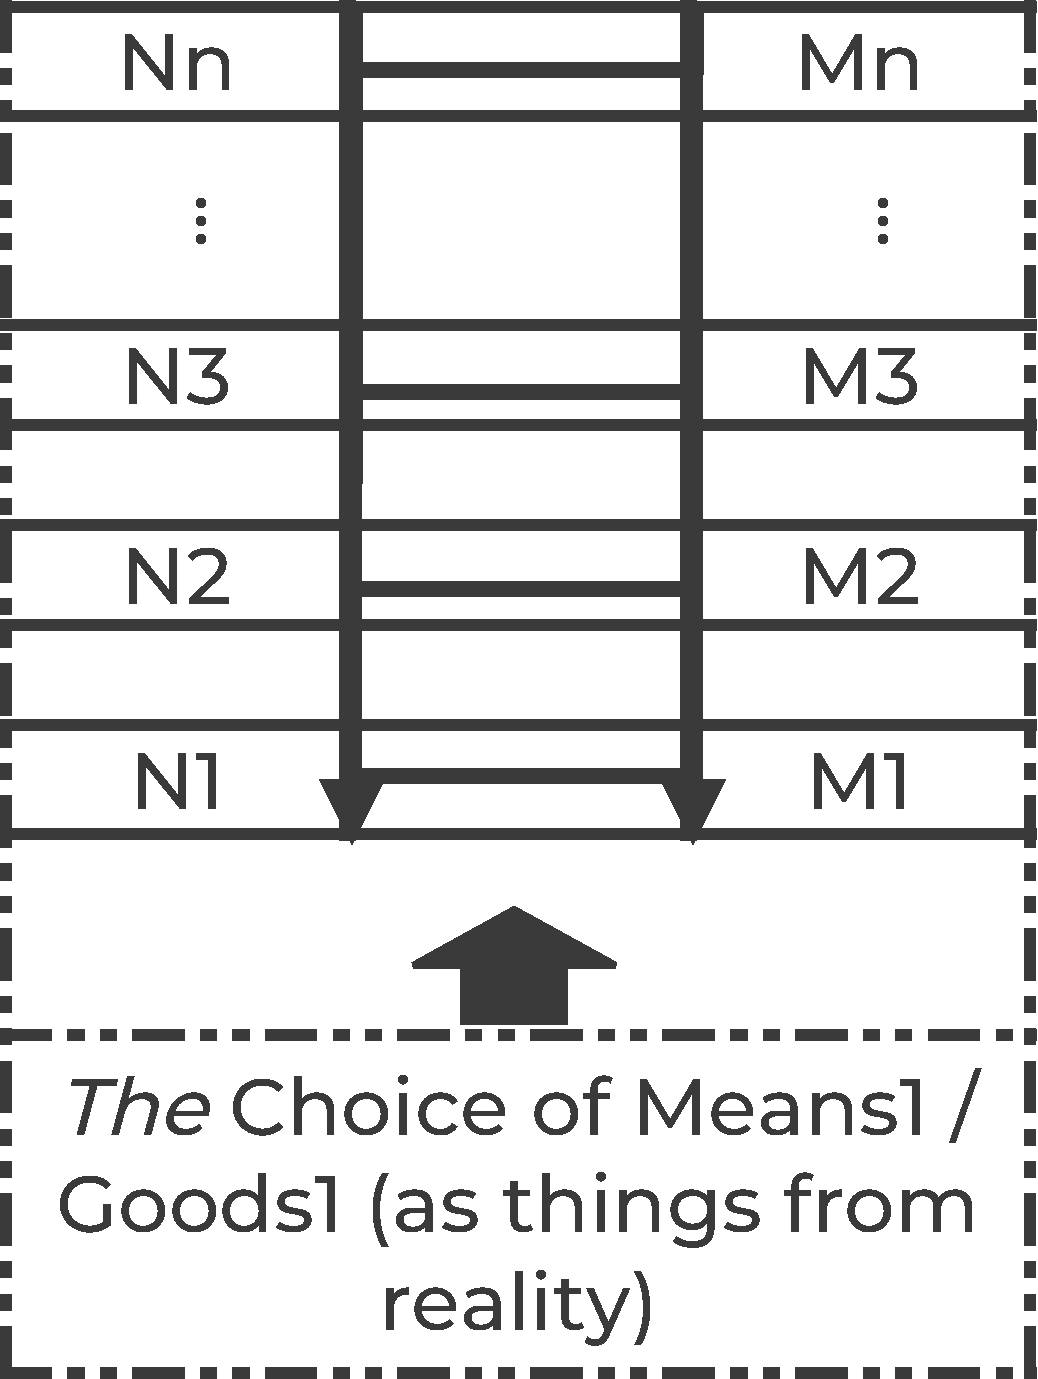
\includegraphics[width=.35\textwidth]{ART_Posvanc/Illustration1_PU.pdf}%
 \end{center}%
 \caption{Consistent neo-Misesian value scale.}\label{pos:fig1}
\end{figure}




The illustration~\ref{pos:fig1} describes the \textit{connection} of the need N1 with the means M1 and it is this connection which is ranked on the scale. Once man (mentally) decides about the most valuable one, he decides accordingly to choose some things in reality and make them economic goods. We cannot have only a~scale of needs on the left side of the ``value ladder'' and non-connected means on the right side.\footnote{It is Biľo 
%\label{ref:RNDOs6YYKfDB6}(2004)
\parencite*[][]{Bilo2004Theory} %
 who tried at least to divide the evaluation process into ex-ante evaluation of ends and then in-action evaluation when we select the most appropriate state of affairs. For a~critique of this approach, see 
%\label{ref:RNDEONR80u8bo}(Pošvanc, 2019).
\parencite[][]{Posvanc2019Evolutionary}.%
} The scaling of an N-M interconnection is necessary. It is important to repeat that it is different if the N1 is defined as going to some cinema, with some wife, and some way, or whether the N2 is defined as going to a~particular cinema, with a~particular wife, and using a~particular way. The interconnection in question, so to speak, defines the need and corresponding means. This isn't a~purely empirical, somehow objectively given, interconnection. It is derived from the agent's knowledge. It is mentally constructed by him to compare his factual and contrafactual \textit{value} possibilities to determine the most important one. However, this would cause a~circularity in the argumentation. Neo-Misesian interpretation namely claims that the value is derived from ranking, but the rank of Ns-Ms already implies a~value link.



The consistent neo-Misesian interpretation of value emergence based on the value scale would be, therefore, problematic, and its circularity is already in our interpretative language. Consider when we say that something is valued more relative to something that is also valued, but just less. We rank within the same class in question (value class) to be able to compare something as more or less valuable. Similarly, in terms of the definition of the concept of cost, we speak of the sacrificed opportunity as the second most valuable alternative 
%\label{ref:RND2AzKBVAaQp}(or ``the next most urgent want'' Mises, 2003, p.174),
\parencite[or ``the next most urgent want''][p.174]{Mises2003Epistemological}, %
 which implies that the second alternative is already valued before the scale creation and it is put as second in the order. Neo-Misesians basically describe a~\textit{ranking} of \textit{attribution of use value} to means/goods to define the \textit{most valuable} one, which manifests itself precisely in particular action. However, the process of arriving at a~given decision and the question of value essence is clearly more complicated 
%\label{ref:RNDyadcewONt9}(see also O'Driscoll and Rizzo, 1996, pp.45–46; Grassl, 2017).
\parencites[see also][pp.45–46]{ODriscoll1996Austrian}[][]{Grassl2017Toward}.%




\section{Proposal to resolve a~paradox }



To resolve the paradox, we need a~new interpretative paradigm of the decision-making process behind valuation and choice. I~claim that we mustn't apply the law to goods per se (which are always particularly chosen), but to the mental order concerning our state of well-being and its marginal changes. This isn't just a~practical solution to avoid particularity of goods. The decision-making process is phenomenal in its nature. The human mind interprets surrounding reality only phenomenally.\footnote{Although the interpretation conducted here is based on Hayek 
%\label{ref:RNDnnzYjuT5mS}(1952),
\parencite*[][]{Hayek1952Sensory}, %
 in my view, there is a~quite vital possibility to connect it to the phenomenological branch of the value theory related to mental states developed by authors such as Brentano, Ehrenfels, Marty, Meinong, Witasek, and others 
%\label{ref:RNDS5MU0XqU1r}(see Smith, 1994; Grassl, 2017).
\parencites[see][]{Smith1994Austrian}[][]{Grassl2017Toward}.%
}



We should start with Pošvanc's 
%\label{ref:RND3ZvY09RO1G}(2021b)
\parencite*[][]{Posvanc2021Problem} %
 attempt to deal with the paradox which provides background for here-presented interpretation. Pošvanc addresses Nozick's challenge by accepting the impossibility of indifference associated with particular choice defended by Austrians. Every action is particularistic and hence so is the value attributed to chosen goods! However, Pošvanc claims that we act in the context of some desired state of ordering of things (portfolio), which provides us with an (admittedly dynamic but still referential) state of indifference. Basically, man would love to have such a~combination of goods which provides him such a~state of affairs that he wouldn't be forced, by felt uneasiness, to intervene by action.



Each choice aimed at acquiring a~good is particularistic and changes the structuring of the portfolio of goods, while the homogenized enduring element of interpretation is the portfolio itself (the whole) and its marginal changes. The more the portfolio is structured in such a~way that we are better able to react with it to the potential removal of the anticipated uneasiness, the more satisfied we are and vice versa. The perceived decrease in the utility of an additional unit of X~is derived from how appropriately/inappropriately the addition of unit of X~in question changes the structuring of the portfolio; basically, the second and third unit of X~causes less and less relevant changes compared to changes made by the first unit of X. At the same time, the disposal of already possessed Y~from a~portfolio as a~good needed to acquire the X, not necessarily as part of the exchange of X~and Y, is part of the interpretation.



It is clear that the portfolio is a~thought construction. Any grouping of goods that we can call a~portfolio would be just a~bunch of things as parts of reality without the agent's mind and his view. It is the agent that ascribes meaning and context to a~given structuration. A~portfolio is thus a~reflection of the agent's Idea of economic orientation where the Idea is the \textit{essence} of the portfolio, which manifests itself in the concrete combination of real goods, which we can call the \textit{substance-based} structuring of reality according to the agent's insight.



The interpretation in Pošvanc 
%\label{ref:RNDx7babpHire}(2021b)
\parencite*[][]{Posvanc2021Problem} %
 is only substance-based in its character. It is an interpreted consequence, but not the cause of the phenomena in question. Some mental-phenomenological-level interpretation must be implied. This is where Hayek 
%\label{ref:RNDULiSzgdAcM}(1952)
\parencite*[][]{Hayek1952Sensory} %
 and especially his analogy of the Map and the Model can serve as an inspiration. One of the reviewers of this paper has rightly wondered whether it is possible to link the analogy in the context of the problem we are addressing. Before I~provide the link, let us briefly look at Hayek's analogy.



\subsection*{Map and Model }



Hayek 
%\label{ref:RNDXQBpA1CvRp}(1952),
\parencite*[][]{Hayek1952Sensory}, %
 in attempting a~conceptual account of the human mind, in my view, applies a~strategy of multi-order-ness: the interrelationships of the neuronal and sensory orders and many layers of mental orders are interpreted as a~new order (new order-whole), which we call the conscious mind. The principles of classification of information (the many-layers-ness of \textit{mental} order) that result from the interrelation of neuronal and sensory orders cause the mind to reflect in a~somewhat identical, but not fully identical way, the order of things in reality; the mind interprets reality and through this process differentiates itself from reality, causing the mind to perceive itself; basically, free will arises as some layer from previous lower-level \textit{mental} layers and develops itself into a~unique personality.



For the purposes of this paper, the analogy between the Map and the Model, which Hayek 
%\label{ref:RND4PVSQH2bFq}(1952)
\parencite*[][]{Hayek1952Sensory} %
 describes primarily in sections 5.17 to 5.91, is important to us.\footnote{The reader should, in my view, be warned to read Hayek contextually when describing this analogy. For sometimes he describes the Map and the Model in the context of any organism and sometimes in the context of the mental order of man. In doing so, he tries to link the mental level with the physically constituted neuronal and sensory order-ness that are driven by naturally defined laws. At the same time, he does not hesitate to remind us from time to time that the emergence of the Map and the Model is subject to the historical evolution of organisms. In other words, he suggests that the proto-origins of the Map and the Model, as well as of mentality as such, are to be sought in the evolutionary development of organisms. So, it is difficult to follow but once a~reader accept that all is deeply dynamic in the description, it should make sense.} The Map is described as a~mental, topological, not topographical, model of the mind (or any organism) of the surrounding reality (like a~subway map), where the various neuronal patterns that organism acquires through experience serve as the ``hardware'' that evokes the Map. The Map is not an accurate picture of reality. Rather, it serves for orientation of the organism in the environment and is created in the context of the environment in which the organism has lived. Although what it has experienced has had a~particularized form, as well as the associated patterns of stimuli must have been particular, the Map is universal in its character; it implies the possibility of combination and associativity of the various ``knowledge'' of a~given organism about its environment, which, according to Hayek's theory, is possible on the basis of the classification of stimuli in terms of an order/group/class. This allows to create some (mental) universals because any order/group/class implies that some phenomena are classified based on some similarities; and yes, it implies that any organisms create \textit{their own} universals to interpret reality. This in turn, meaning creating universals based on the classification, allows for the association of past experience to similar, but particularly novel, circumstances through which the organism grasps the reality. The Map is constructed on the basis of experience in a~gradual manner, where the later stimuli must be incorporated into the Map in the context of earlier ones; and also, many different maps of organisms evolve as species does. Hayek goes so far as to say that the analogy of the Map fades away gradually 
%\label{ref:RNDmKrYtgcrms}(Hayek, 1952, sec.5.30),
\parencite[][sec.5.30]{Hayek1952Sensory}, %
 and this is because what we are describing creates more and more new layers of classification.



The Model ``grows'' over the Map. It is predictive. In the context of less evolved organisms, Hayek describes a~Model as based on associativity of neuronal activity, which allows for the application of a~combination of patterns to new anticipated events, where the Model prepares the organism for various contingencies that may come based on cues from reality. Hayek writes 
%\label{ref:RND603axN6tkf}(Hayek, 1952, sec.5.87):
\parencite[][sec.5.87]{Hayek1952Sensory}: %
 ``Whenever the classifying mechanism treats as alike, or as alike in certain circumstances, any group of events, it will be able to transfer any experience with any one of them to all of them.'' The Model is therefore more robust and richer compared to Map. The reason for this is the universality of classification, where, on the basis of universals arising as (spontaneous\footnote{Interesting in the context of spontaneously arising thoughts is the research on the influence of the REM phase of sleep on people's mental states, which is manifested in the context of the brain seeming to integrate some cognition on its own without the deliberate action of consciousness (the so-called Eureka effect); see, e.g., Pstružina 
%\label{ref:RNDSvGAYSC7Th}(1994).
\parencite*[][]{Pstruzina1994Etudy}.%
}) products of classification, the Model allows the construction of broader circumstances that the Map doesn't and cannot contain. But at the same time, the Map and the Model influence each other. Changes in the Map affect changes in the Model and vice versa. These are thus semi-permanent dynamic structures 
%\label{ref:RND8TBCl8FwvK}(Hayek, 1952, sec.5.43).
\parencite[][sec.5.43]{Hayek1952Sensory}. %
 This means that if the Map did not contain some universals before, the influence of the Model causes the Map to develop in that direction. This results in the Model being able to combine and model new eventualities more robustly.



Although Hayek highlights the influence of the past on the construction of the Map-Model, it should be noted that the context of the Map-Model's continued operation is not tainted by the influence of the past. The past provides stimuli that are classified universally, which in turn allows for associativity, new forms of combinations in the classification of stimuli, or the predictability of the Model. Although the Map 
%\label{ref:RNDizY418Zkf5}(Hayek, 1952, sec.5.42)
\parencite[][sec.5.42]{Hayek1952Sensory} %
 represents a~picture of the past in which the organism lived, it does not in itself provide information about the current state. Thus, the past is relevant only in the sense that it provided the stimuli for the construction of the universal Map, but the whole mechanism of the Map-Model is oriented towards the future. And this, according to Hayek, is true for all kinds of organisms 
%\label{ref:RND3kDu4OqT06}(Hayek, 1952, sec.5.61),
\parencite[][sec.5.61]{Hayek1952Sensory}, %
 not just humans.



From the human point of view, the basic characteristics of the Map and the Model are already incorporated (evolutionarily) in the genetic equipment of man in the form of various kinds of automatisms (mechanical, instinctive behavior), which are subsequently developed into the abstract-mental form of the conceptual and conscious mind. However, many operations of the brain and mind remain at the level of automatisms, and only a~minor part of the phenomena remains in the attention of the conscious mind. The mind does not classify objective reality as it is (as a~thing-in-itself), but only in the context of a~pre-existing classification by classes of other objects of reality, when conceptual knowledge is formed as the formation of abstract concepts at higher levels of the informational and mental order. In the sense of the conscious mind, this permanent classification and reification according to Hayek 
%\label{ref:RNDLDK10F7Zn0}(1952, sec.6.47)
\parencite*[][sec.6.47]{Hayek1952Sensory} %
 comes crashing down on us, because this classification is still only an inaccurate representation of reality.



\subsection*{Map–Model and the Idea of economic orientation (portfolio) }



Having briefly introduced the analogy, we can, \textit{mutatis mutandis}, proceed to realize the link between the analogy and the above-mentioned \textit{Idea of economic orientation.}\footnote{As a~supportive argument to the here-presented attempt, we could use Horwitz 
%\label{ref:RNDT9NT6HZ3U6}(2010),
\parencite*[][]{Horwitz2010Sensory}, %
 who followed a~similar approach to deal with an organizational learning problem using Map and Model as an explanation of Balance Sheets and Budgets. The Map and Model are essential phenomena to mental structuration of Balance Sheets and Budgets while Balance Sheets and Budgets reflect or represent a~real structuration of the historic activity (Balance Sheets/Map based) and planned activity (Budgets/Model based) of the firm within a~reality.} The Idea of economic orientation transpired into the portfolio concept is not the \textit{whole} Map–Model dynamics, but it is possible to consider it as some mental sub-order. The Idea, as a~sub-order, has all the characteristics of the Map–Model analogy: 1) The portfolio of actually owned (acquired-spent) goods is nothing else than the result of the person's past economic ideas and experiences. It thus reflects a~coherent \textit{universal} Idea of a~person's economic experience within his or her environment. 2) Some future–oriented state of affairs constructed as a~picture of desires and needs transpired into the desired portfolio has an anticipatory (Model–based) character. It expresses what we would like to have in order to be able to face an uncertain future.\footnote{As Pošvanc 
%\label{ref:RNDutiARrmACG}(2021a)
\parencite*[][]{Posvanc2021Evolutionary} %
 shows, we do not prepare for future precisely, as if in all possible details. On the contrary. The predictiveness is based on relativizing the meaning of the particular state of future through the combination of means and diverse features of them with each other, reshaping and combining physical properties of things in a~way so that a~given different combinations of needs to be fulfilled are ``embedded'' in things/goods (e.g. steel is transformed into a~knife in such a~way that it can be used to cut meat, but also as a~weapon or a~tool for carving toys), as well as the evolutionary discovery of the universal characteristics of individual needs and the associated features of means (area of entrepreneurship), and last but not least, the construction of various economic tools through which we communicate this knowledge to each other, such as, e.g., money, or the price system providing information about bid-ask spreads, but also various social institutions guaranteeing universals for our orientation in reality in the form of, e.g., property rights or law enforcement we can rely on in the time continuum.} 3) There is also a~potential state of affairs which expresses what we can realistically achieve as kind of combination of the Map and Model universal knowledge.



The interpretation should start with our idea of how something ought to be (Model–based Idea). This normatively defined Idea is as if some ``picture'' about the desired state of well-being which is confronted with how something is and how we are able to (based on the knowledge) achieve the state in question (Map–based Idea). It is a~flexible–dynamic mental structure of desires and needs present as some future picture of state of affairs,\footnote{This image is made up of both real and unreal ideas.} to which flexible–dynamic mental structure of combination of means of their fulfillment is formed (the Idea of a~desired portfolio).



The Map part of the structure consists of an actual and a~potential idea of the portfolio. The reason to think about them in the area of Map is twofold: a) the Map structure has its correspondence/reflection into the real world as a~substance-based portfolio of real goods.\footnote{I~think that this is also the way how free will (as pure phenomenon) exerts causal influence on the noumenal world (thing-in-itself); by \textit{correspondence} or by \textit{reflection of this correspondence}.} It informs us about existing combination of means; what we really have as the existing portfolio in t\textsubscript{0}, b) the Idea of the potential portfolio always happens to be the actual one in t\textsubscript{1} and the change must happen in reality as well.



However, the knowledge of what we can attain as some potential portfolio in some defined t\textsubscript{1 }is as part of the Map (universal knowledge based on experiences) as well as of the Model (prediction–based knowledge). The mental decision to change existing combination of means and our ``problematic'' particular subsequent choice of a~real good is merely a~boundary state by which we change our overall portfolio in the reality, which subsequently causes actualization of the Idea of the portfolio within a~mental Map structure.



The interpretation has also led us to the wanted homogenous element which provides a~reference to indifference. It is the Idea how a~\textit{combination} of needs could be fulfilled by a~\textit{combination} of means (portfolio); or the Idea of economic orientation\footnote{It is not purely Kantian subjective kind of Idea. The Idea is also influenced by naturally given automatisms of men (e.g., instincts) and the socio-cultural intersubjective context and could be, therefore, interpreted better as part of Hegelian evolving Absolute Idea 
%\label{ref:RNDw94dhyAF3H}(see interpretation of Hegelian logic by Harris, 1983).
\parencite[see interpretation of Hegelian logic by][]{Harris1983Interpretation}. %
 }. Due to the Model–Map analogy the Idea is triadic: as the Idea of \textit{desired---actual---potential} portfolio; This mental structure persists, although it is still different, which is caused by different interconnections and combinations throughout time; if we use Hegelian expressions, what is achieved, as a~potential portfolio, sublates (German \textit{aufgehoben}) over what was desired and what was actual.\footnote{The explanation of the logic behind the Triad; see Maybee 
%\label{ref:RNDMoaGPUfvG8}(2020)
\parencite*[][]{Maybee2020Hegels} %
 or deeper analysis e.g., in Harris 
%\label{ref:RNDgGoIHSGetw}(1983).
\parencite*[][]{Harris1983Interpretation}.%
}



We can imagine it as the very simplified illustration~\ref{pos:fig2}: I~have illustrated separately the Map and the Model in order to illustrate the differences, but a~given Idea is the one coherent mental whole, where the desired and potential states are only imagined and compared to the actual state in reality based on the combination of knowledge of how to achieve the states of affairs in question; the illustration~\ref{pos:fig2} can also be imagined in such a~way that the given geometrical objects lie on top of each other as layers, which would equally illustrate the differences and at the same time they would be one dynamic geometric figure.


\begin{figure}
 \begin{center}
 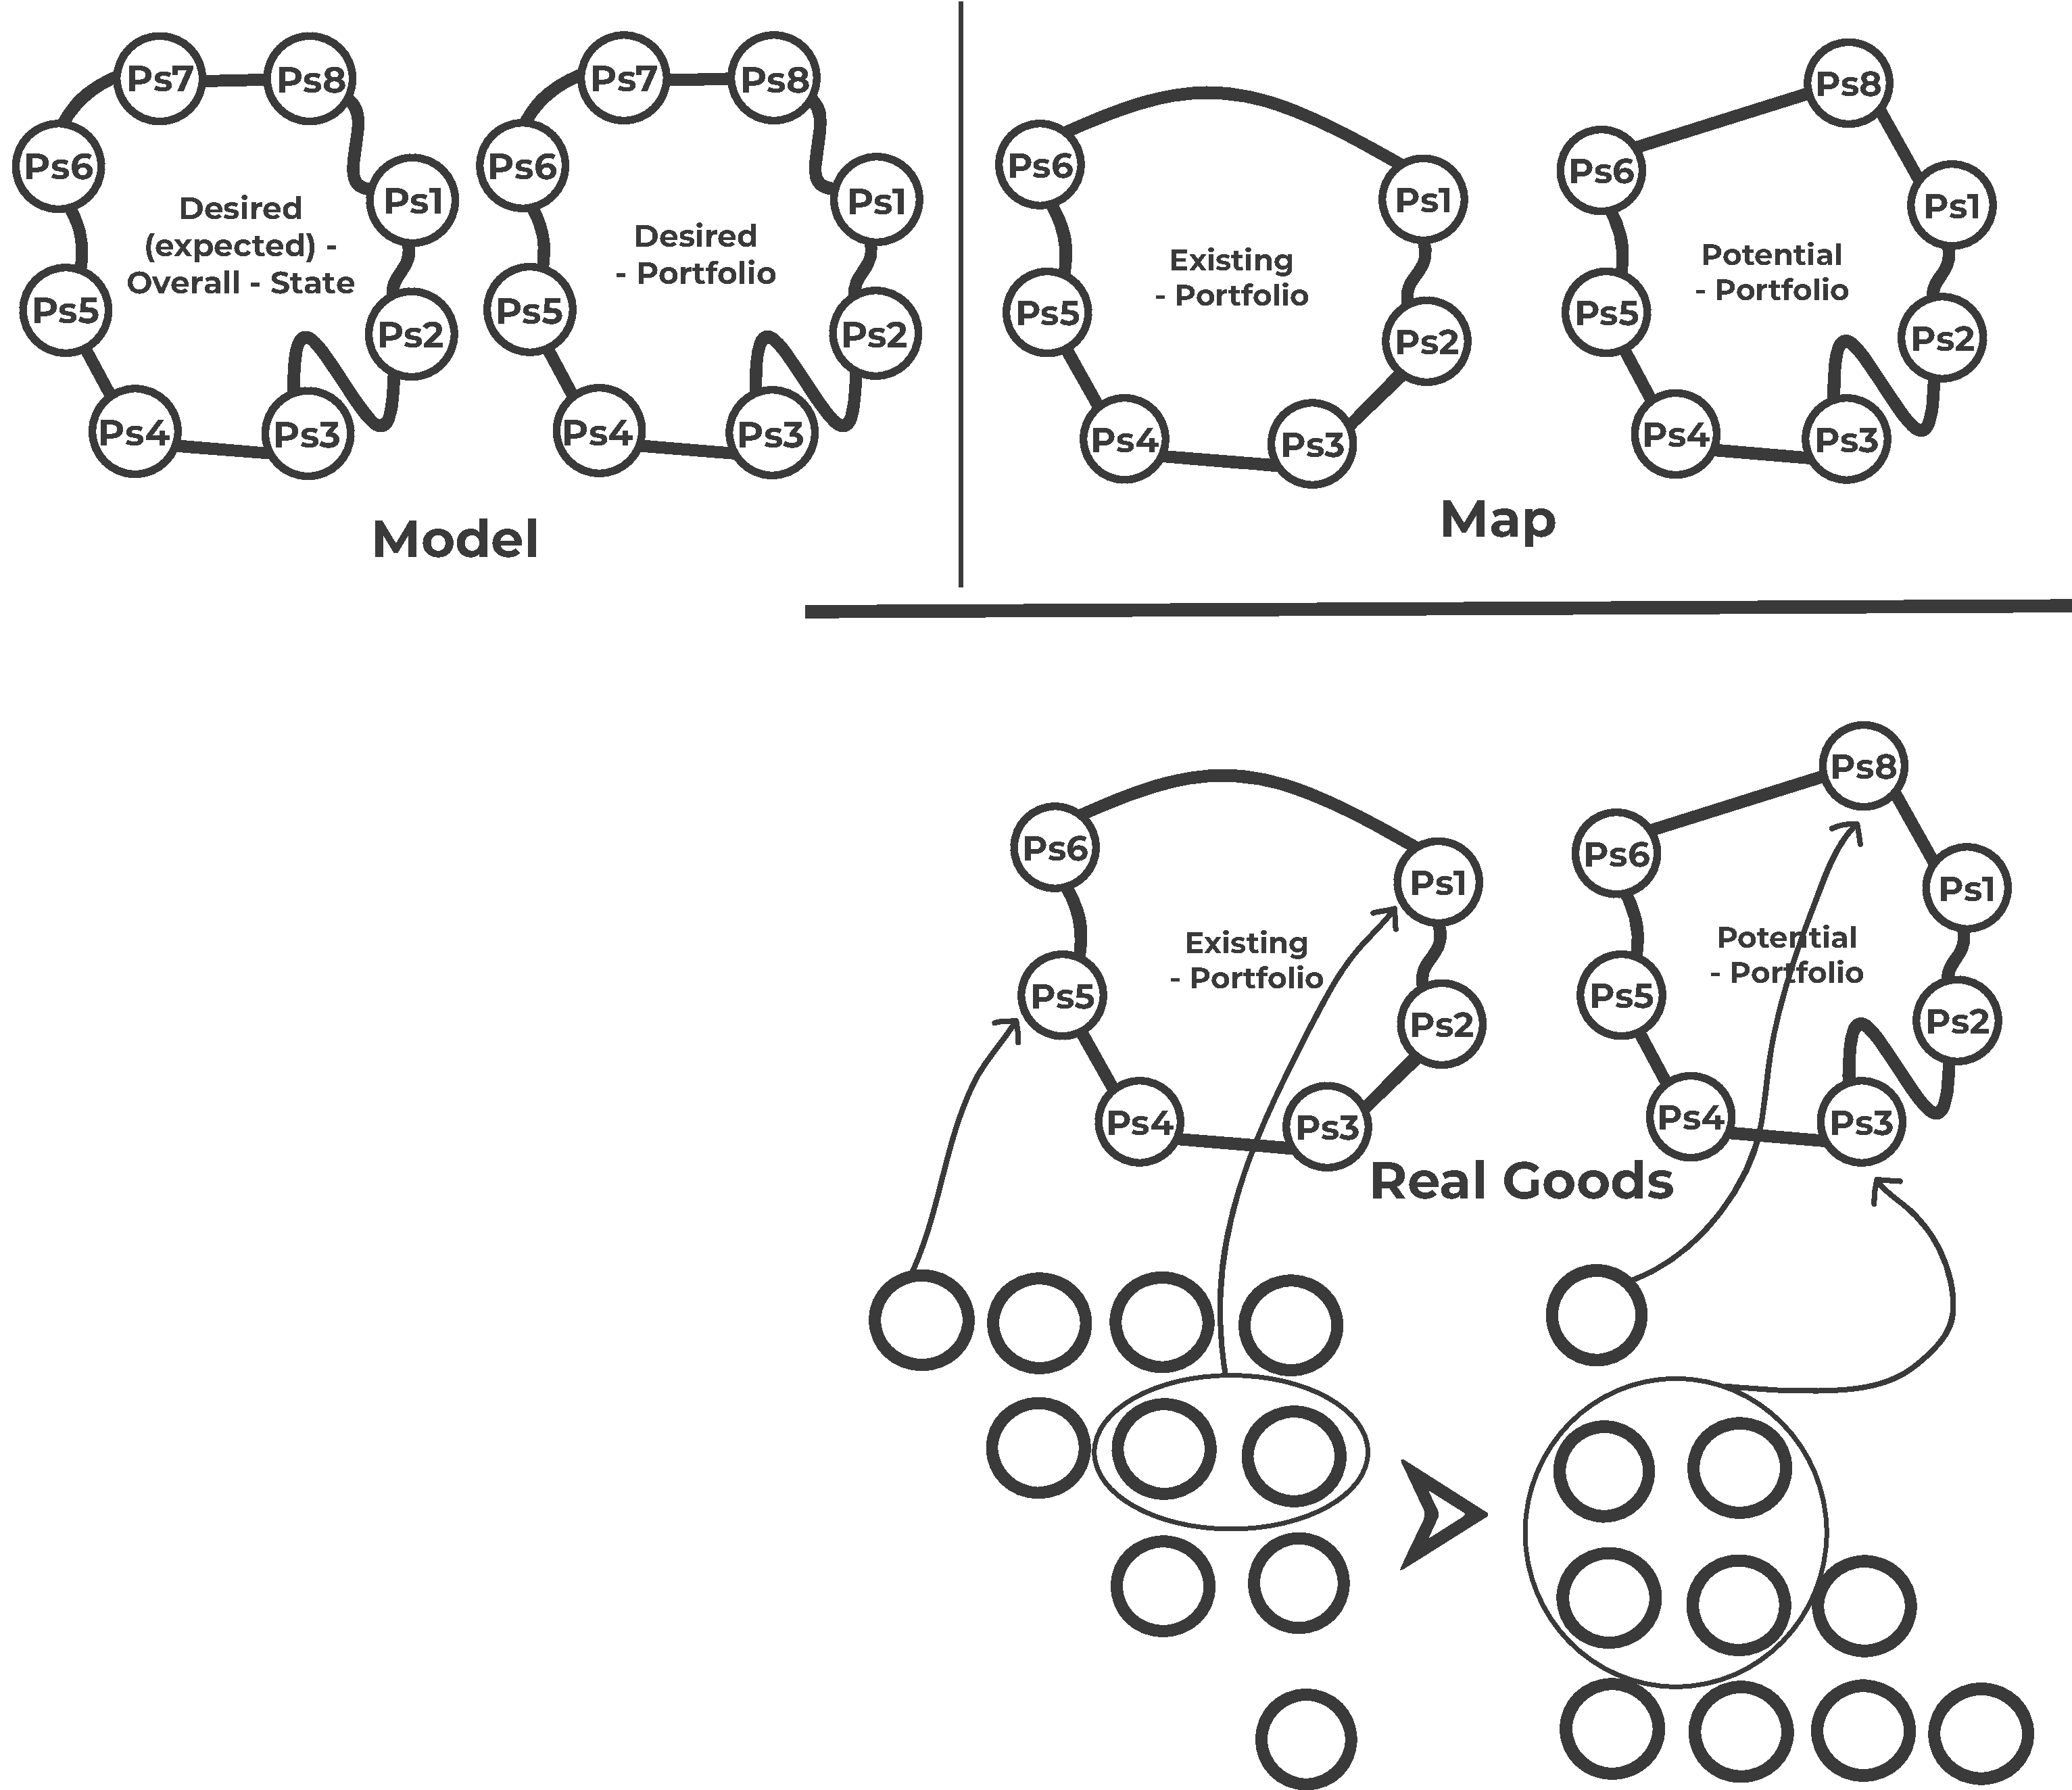
\includegraphics[width=1\textwidth]{ART_Posvanc/Illustration2_PU.pdf}%
 \end{center}%
 \caption{Man's idea of economic orientation.}\label{pos:fig2}
\end{figure}






I~illustrated mental structures also consisting of some partial states (Ps)---these states are like puzzle–parts of the whole picture of man's Idea, and they could represent personal ideas about anything, e.g., my idea about accommodation, food, work, leisure, holiday, socializing, etc. Basically, partial ideas of what different aspects of a~person's life should be like.



We can see illustrations of a~Model–based Idea (top left) and a~Map–based Idea (top right). Bellow the line are real goods (as circles) composed into the real existing and the potential portfolio; existing one would be changed into the potential one based on action; desired one is unreachable as a~kind of ideal state.



A~Model–based Idea as a~future–oriented mental state is a~dynamic---reference---state of affairs. It is composed of partial states. The Model models our ideas in the form of needs and puts them together with some ideal combinations of means (some ideal portfolio). It is illustrated by the correspondence of Desired state of affairs (as needs and desires) and Desired portfolio of means. This thinking could be about real or imagined connections between needs and means 
%\label{ref:RNDvKMUNx4jG1}(Menger, 2007),
\parencite[][]{Menger2007Principles}, %
 e.g., as part of the whole structural picture of all my needs, there could be some structural partial-need-state in the form of an idea of my ideal house connected to some idea of a~beach house with a~swimming pool and surfing possibilities. But the model can also produce totally imaginary partial needs, such as the desire to be able to do magic interconnected with the idea of a~magical wand in the context of the whole picture of man.



A~Map–based Idea of Portfolio (as a~mental state) is actually an idea of how something is at time t\textsubscript{0} (represented as what we already have as an existing portfolio of means, e.g., I~don't have the dream-house but I~have a~car) and what it is possible to achieve at time t\textsubscript{1}, e.g., I~can have some kind of knowledge of how to achieve my dream-house or just to make some kind of compromise, e.g., I'll just settle for a~holiday in a~house like that. A~Map-based Idea of Portfolio is changed based on the knowledge transformed into the plan about how to combine existing and new means implemented as action from time t\textsubscript{0} to t\textsubscript{1}.



The change is illustrated by the difference between the structure of the existing portfolio and the potential portfolio (a new partial state, P8, is illustrated and constructed, and the shape–line of P2 and P3 was changed to better represent the correspondence to the desired portfolio caused by a~new kind of combination of means). Basically, the point of the illustration~\ref{pos:fig2} is to show that the existing portfolio structure is more different than potential portfolio, and the non-correspondence is the motivation to act and improve the state of affairs.



The real portfolio is what I~have as real things, e.g., parts of my real accommodation, what I~eat, where I~work, what kind of leisure I~enjoy, where I~go on holiday, who my friends are, etc., and potential portfolio represents what I~am able to achieve. The potential portfolio is constructed by action and is always more similar to the desired portfolio we ideally want to have. So, to improve my state I~have to act, for example, by buying some accommodation to have my house to be more similar to my ideal idea. The potential portfolio represents our ability of what we can achieve under the constrains of individual knowledge, meaning that I~can desire Iron Man house-style on the beach, but my knowledge is inadequate for achieving this desire, so I~have what I~can afford.



The movement from an existing to a~potential portfolio is therefore both a~mental process as well as a~real act; in red there is indicated a~(action/choice) selection of real things---goods, which we combine and group/compose into a~new portfolio that will change its character within reality and thus in the mental area of the Map.



It follows that man senses the \textit{range of the uneasiness} by how much the desired portfolio doesn't correspond to the real portfolio, and he removes the uneasiness by action 
%\label{ref:RNDbpJoHRBdp9}(compare to Hayek, 1952, sec.5.69 and 5.70).
\parencite[compare to][sec.5.69 and 5.70]{Hayek1952Sensory}. %
 The value is derived from the range of the non/correspondence between the Model and the Map–based Idea of correspondence of mental states. If we choose a~real good and add it to the portfolio, it improves the map-model correspondence, and so we assign a~value to that good or a~bunch of goods in question.



The value then depends on what and how something improves the spread among the Idea of desired---actual---potential portfolio:


\begin{figure}
 \begin{center}
 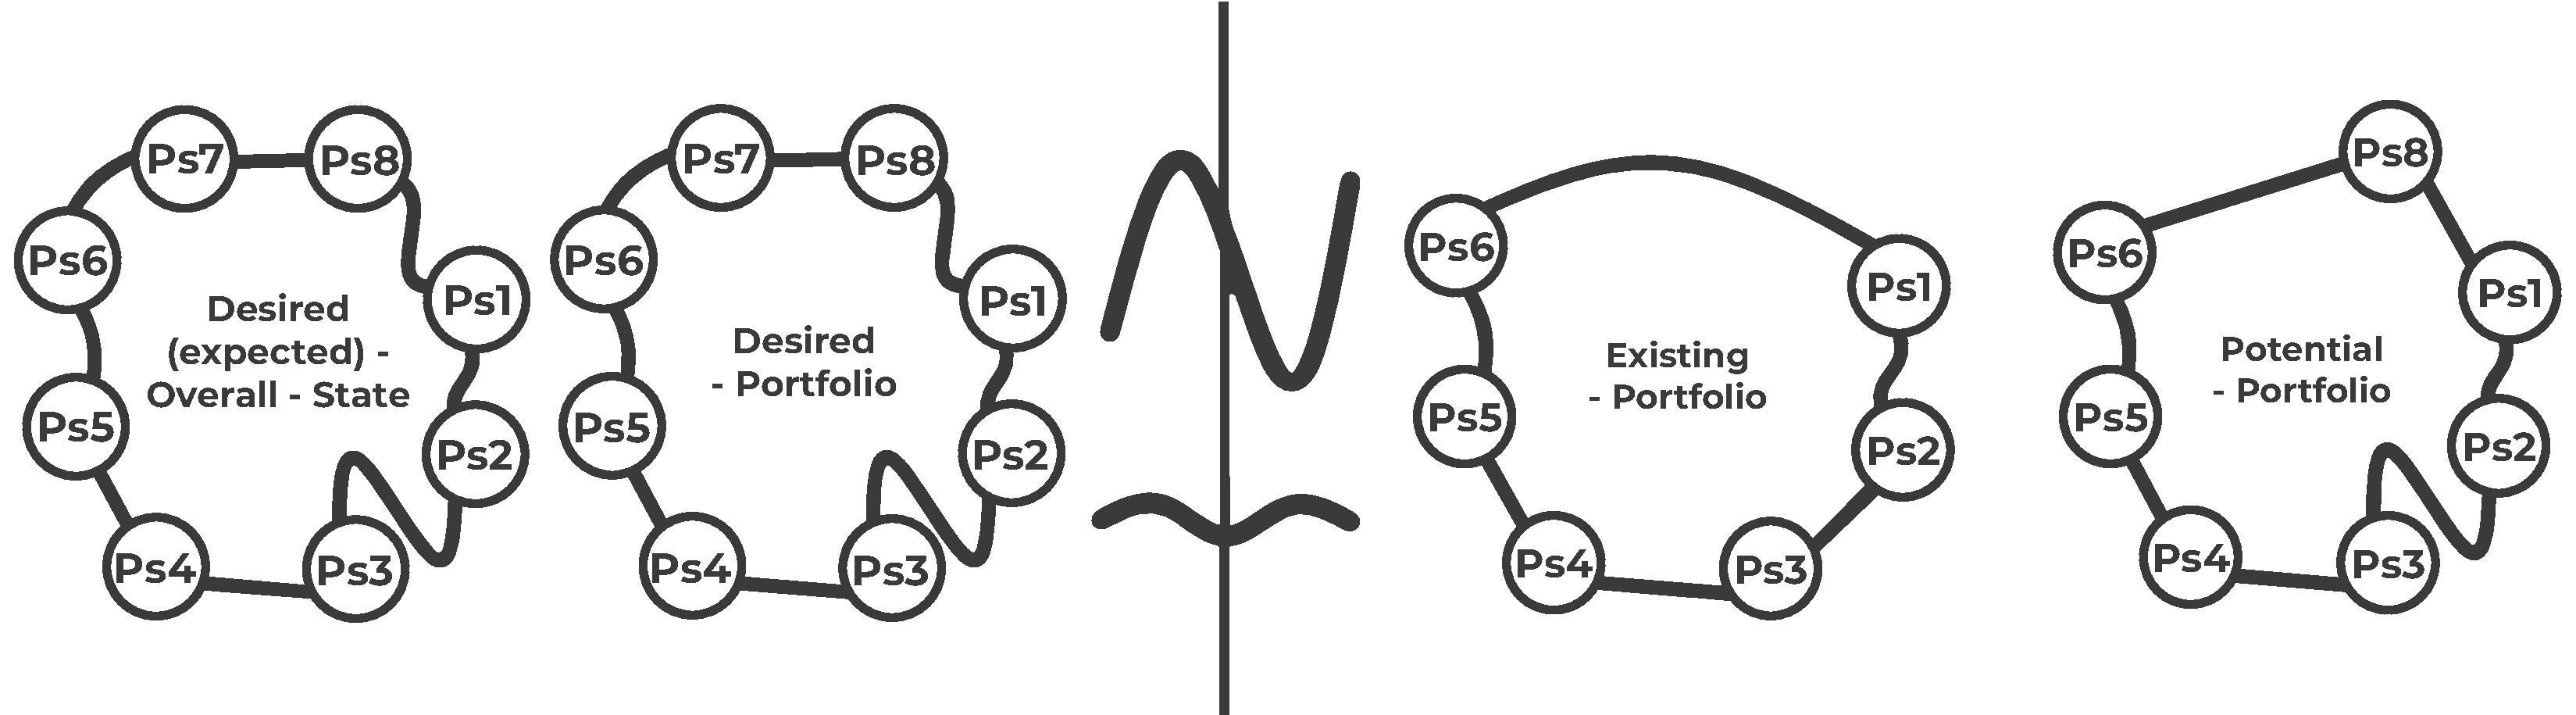
\includegraphics[width=.99\textwidth]{ART_Posvanc/Illustration3_PU.pdf}%
 \end{center}%
 \caption{Subjective value.}\label{pos:fig3}
\end{figure}



So, when we implement a~plan, we try to implement it in the way that the Map Idea of Portfolio corresponds as closely as possible to the Model Idea of Portfolio, and it happens based on what kind of goods we add to the real portfolio; more suitable (valuable) the goods, the higher the correspondence. It has to be stated that these are \textit{also dynamic phenomena:}\footnotetext{ In fact, in the thus-presented context, we can also speculate about more enduring sub-states of the mental structure, which are created intersubjectively (beauty, love, traditions, …), but also of an individual nature (individual habits, stereotypes). }

just as the Model changes the Idea, so do the requirements for the changes/alterations to Idea within the Map (as an endogenous change), as well as the real combinations of goods in reality. The changes happening in reality outside of one's purview have the same consequence on the whole dynamism (which is an exogenous change, however, still mentally grasped).



\subsection*{Response to the Nozick's challenge}



The triadic Idea of ``desired---existing---potential portfolio'' is a~mental construct that is on the one hand a~homogenized whole, and on the other hand, it is (constantly) changing in its particular form with respect to the strictly directed action being performed. Here lies, therefore, also the proposed solution.



We act particularly while striving to achieve a~state of satisfaction (as some homogenized whole), where, in the case of a~coincidence between the combination of needs (as a~mental state) with the combinations of means to satisfy them (as a~mental state) and the real perception of the achievement of the combination of goods (as real things), the agent is indifferent to further action; his mental state of satisfaction is achieved precisely through the achieved combination of goods in reality. He would be in an economic rest.



The homogenized element necessary for the application of the law isn't, therefore, some value-homogenized class of goods. It is instead the perceived mental order between the Model and the Map–based Idea of portfolio and its correspondence with the state of affairs (goods composed into the portfolio) in reality. The correspondence doesn't have to be achieved because of the dynamism of both, but it is possible (at least in some moments of man's life, as we will see below). If the correspondence is reached, it is a~state where we would be in the maximal mode of indifference or a~personal equilibrium and so without having any interest in any new action.



As noted by one reviewer: Can we just rephrase Nozick in the way that ``the homogenized element is not some homogenized class of goods but instead the mental state of indifference against those goods''?. Possibly, but we must add a~necessary condition. The mental state of indifference against those goods is determined on the basis of \textit{internally} perceived \textit{relative} relationship of goods in question to other goods \textit{already perceived} within the actual portfolio.\footnote{Cf. with Wysocki's 
%\label{ref:RNDJzMMKCwqyR}(2021, pp.26–27)
\parencite*[][pp.26–27]{Wysocki2021problem} %
 critique of Block where he made an important point about ``a particular state of affairs (as specified in extensional terms)'' and ``a content of the actor's intention''.} What is relevant here is not only the frequency and interrelations of goods, but also the significance they acquire in their relative positions to each other in the \textit{context} of Needs satisfaction. If we use the geometrical illustration~\ref{pos:fig2} to show this point, what is \textit{also} important is the mereological structural arrangement, determined by subjective details the agent \textit{intentionally} thinks about or which the agent \textit{implicitly} follows based on some wider socio–cultural context.\footnote{This context used by the agent is embedded in linguistic structures, structures of social institutions, or is part of various automatisms created by the Nature in the form of instinctive human reactions or intentionally in the form of, e.g., product design or the provision of contractual services. This context is quite interesting because it is defined for a~subjective decision making in \textit{extensional terms}. Cf. also with the footnote No.3 about radical subjectivism and Wysocki's 
%\label{ref:RNDAWSS5Qr25y}(2021, pp.26–27)
\parencite*[][pp.26–27]{Wysocki2021problem} %
 critique of Block.}



There could be, therefore, a~partial and a~maximal indifference. The partial one is concerned with some sub–partial–Idea of the state of portfolio. Maximal (theoretical) indifference is actually zero uneasiness, or a~state of rest, or total economic peace 
%\label{ref:RNDXGu6A77pKl}(as described by Mises, 1998)
\parencite[as described by][]{Mises1998Human} %
 where we have no tendency to \textit{consciously} act; just automatically repeat reached success and enjoy satisfaction.\footnote{Mises describing these states within his concept of ERE was probably inspired here by Knight's notes about uncertainty or action under certainty and perfect knowledge; see Knight 
%\label{ref:RNDTkRGXaNCib}(1964; 1921, pp.201, 268, 294).
\parencites*[][]{Knight1964Risk}[][pp.201, 268, 294]{Knight1964Risk}.%
} Pošvanc 
%\label{ref:RND3MJFc6xxKI}(Pošvanc, 2021a, pp.203–211)
\parencite[][pp.203–211]{Posvanc2021Evolutionary} %
 doesn't describe this theoretical maximal state as a~state of human–to–robot change, as Knight's or Mises's interpretations might imply, but as a~state of individual satisfaction when we seek to rely on pre–set–automatisms, e.g., contracts or automated provision of services and goods. We would feel full satisfaction or satisfaction at some (very theoretical) maximum.\footnote{The reader should be aware that as Mises / Rothbard did, so here-presented description of a~state of rest is used as some kind of theoretical mental construct.}



While we may never achieve it from a~praxeological point of view, we need to know it in order to get this information by differentiating between what is (existing), what we can achieve (potential) and what we desire (ideal) in some subjective state of ours. Acting causes a~lessening of the uneasiness that comes from the Model–based Idea of portfolio not corresponding to the Map–based Idea of portfolio. In fact, by not conforming to the Map Idea, the Model Idea is actually providing us with information that we need to change something in order to achieve the normatively determined state we want. The application of the law, based on the indifference within the decision–making process which leads into the particular action, can then be illustrated as follows:


\begin{figure}
 \begin{center}
 \makebox[\textwidth]{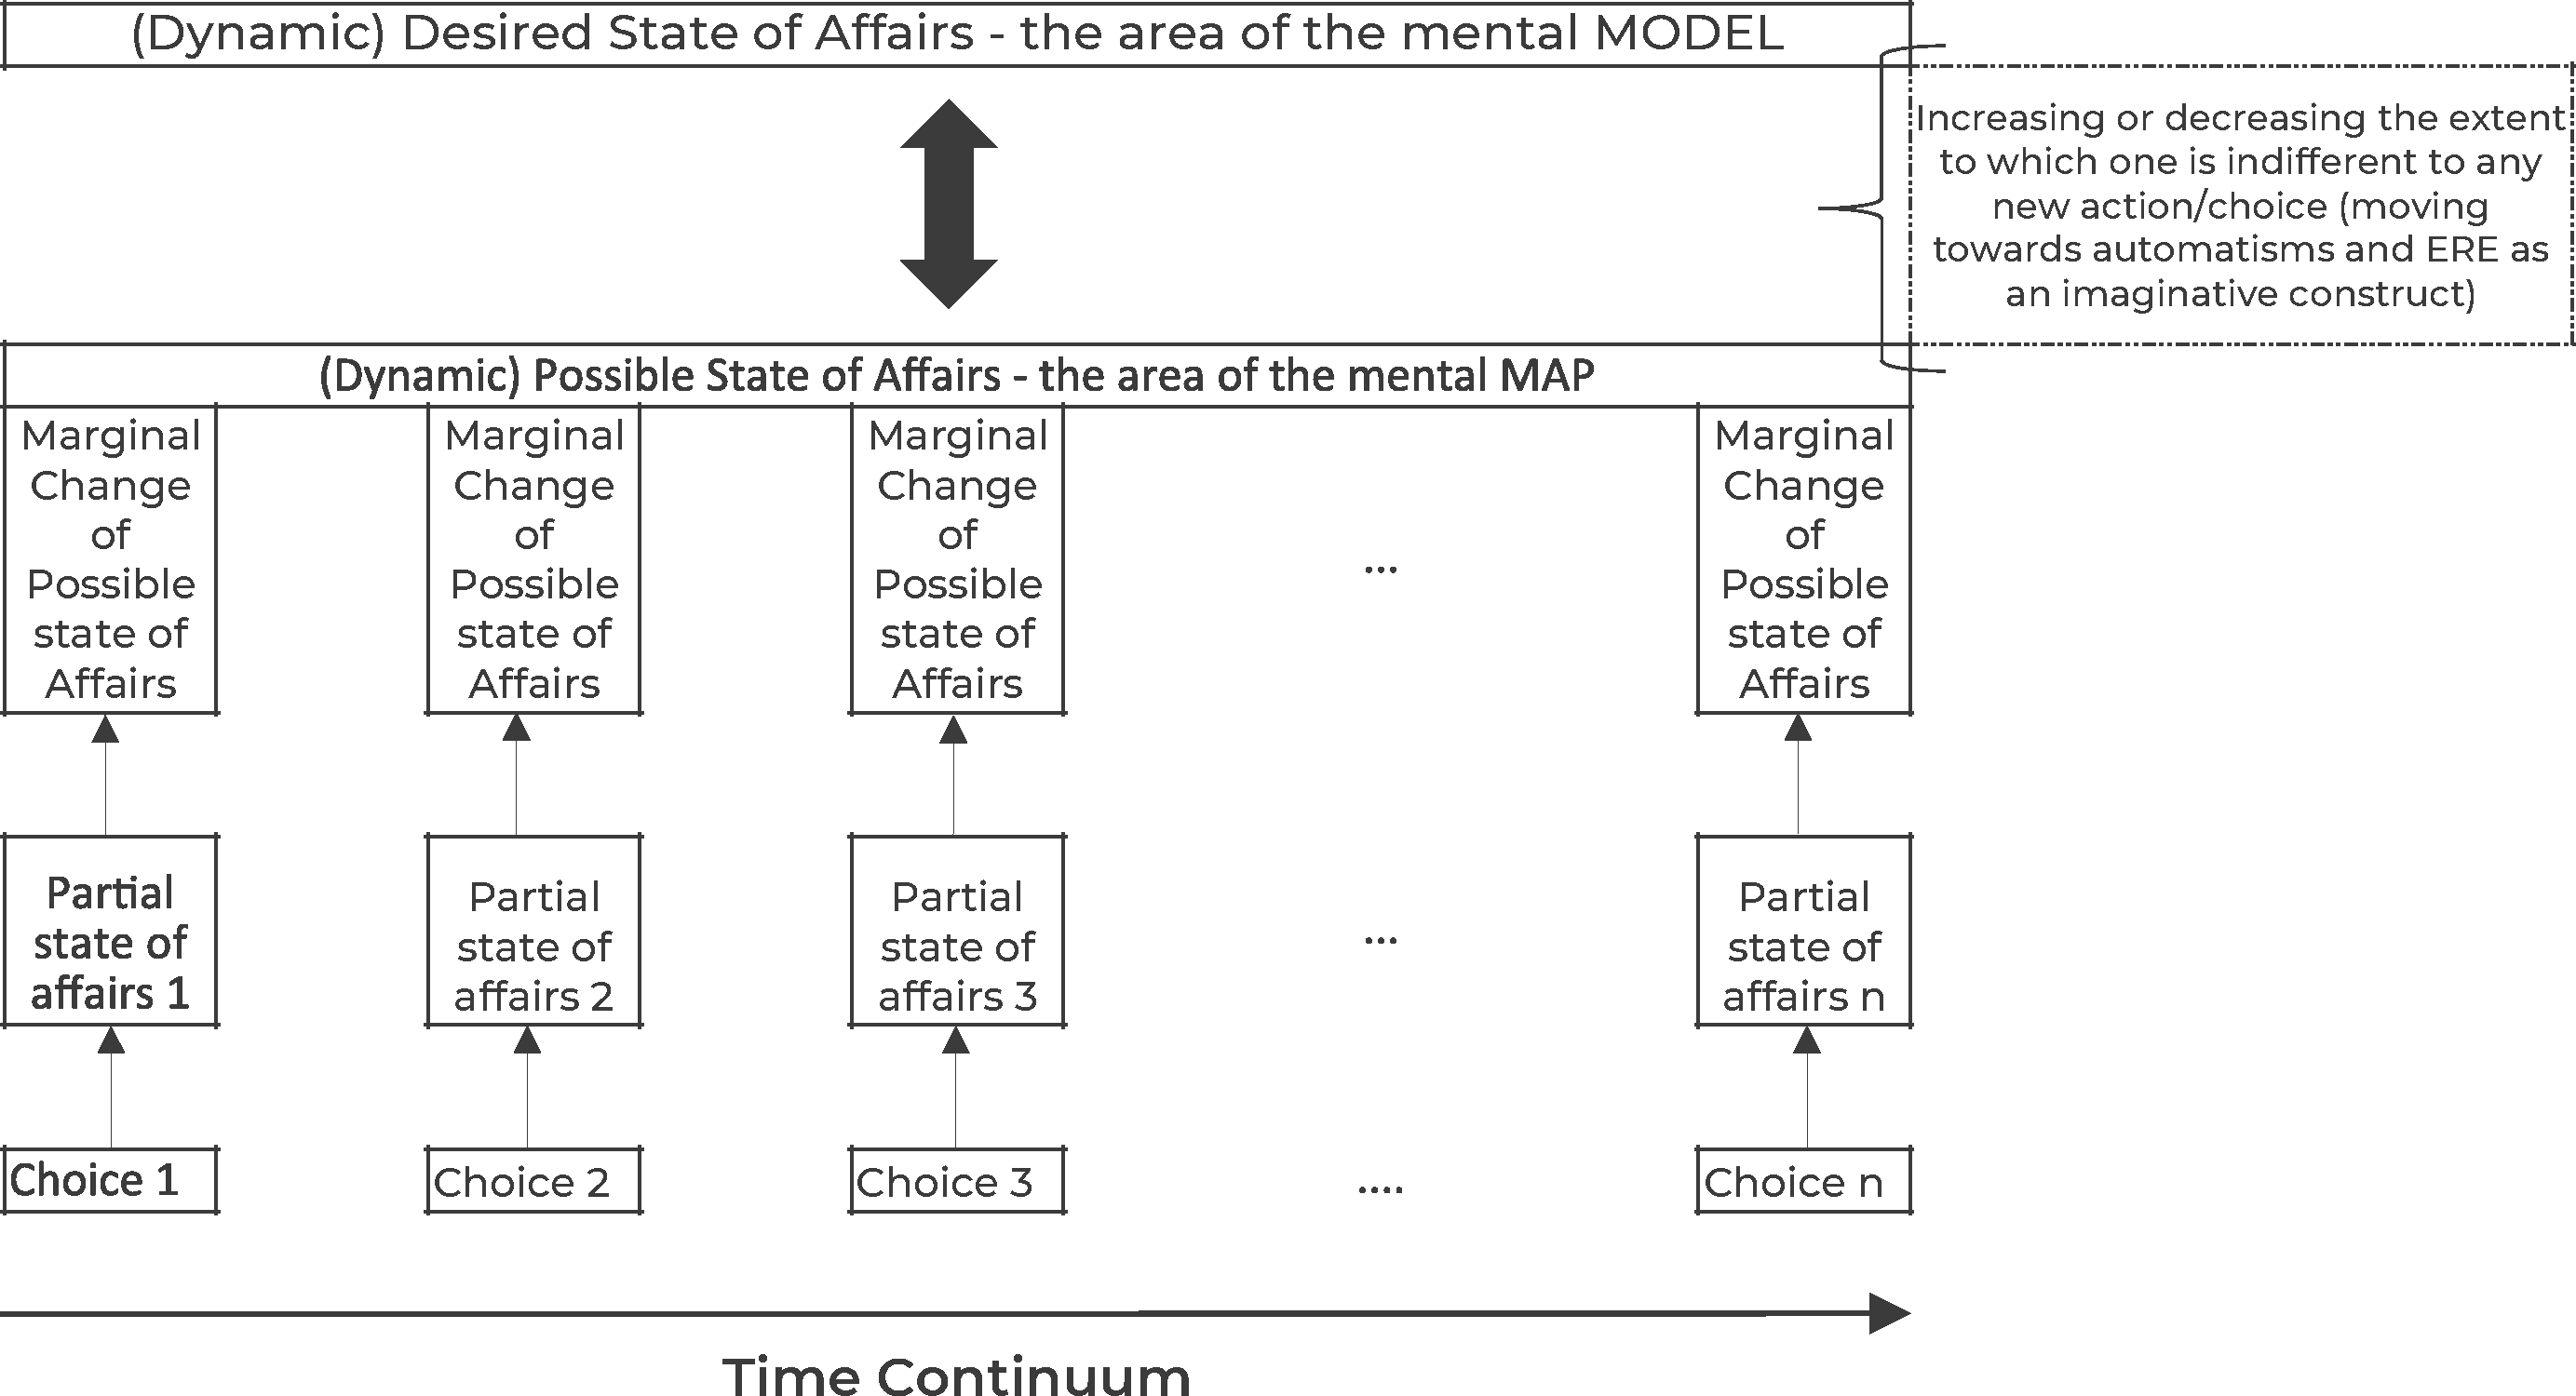
\includegraphics[width=1\textwidth]{ART_Posvanc/Illustration4_PU.pdf}}%
 \end{center}%
 \caption{Law of diminishing marginal utility and indifference.}\label{pos:fig4}
\end{figure}






The illustration~\ref{pos:fig4} shows that we act in a~time continuum. We are trying to reach some \textit{desired state of affairs} where we would be indifferent to any new action. But we are able to achieve only \textit{possible state} \textit{of affairs}. Choice by choice we change the perception of what we can achieve. Each choice contributes to some marginal change in the \textit{possible} \textit{perceived state}, and each choice directs us to make the difference between the desired and potential states as small as possible (acting is intended as if to narrow the space between the desired and possible state of affairs in the illustration~\ref{pos:fig4}). Given that both states are dynamic phenomena and constantly changing, the given isn't attainable (but theoretically possible).



One of the reviewers expressed an interesting critical doubt about the proposed solution; he writes: ``the mental state is reached after the choice is made and needs are satisfied, while according to Nozick, it is the state before the choice which indicates the sameness of the goods.'' It could look like I~have shifted the meaning of the crucial term. It is a~proper point.



However, this is not a~changing of order of events–explanation but a~different level of description; I~modified the interpretation in a~two–level way. The homogenized whole (as if the utility denominator or the ever–present reference state) is the triadic Idea of a~portfolio (or mutatis mutandis a~sub–state of a~portfolio) and each choice within which subjective cost–gains are included just carries particular information about the utility change\footnote{Whether it is possible to define a~unit of utility (util) as some kind of nominator is a~topic that requires separate attention and I~reserve it for a~different paper. }.



A~definition of the indifference concept within this new context is, therefore, a~measure of order–ness of the order (system) in question; in the case of a~human being---range of economic order–ness or peace. Indifference is thus anchored in a~time continuum, always prior to action, but, at the same time, continuously perceived. It is like a~referential maximal state that we never reach, but perceive. We, therefore, act particularly, but always in the \textit{context} of the law; each action increases our marginal state of satisfaction, or ex post we find out that some action was erroneous. We know this based on the spread between desired and potential state of affairs we want to achieve. Once the spread is depressed, we marginally increase satisfaction and vice versa. It is also evident that choice is always a~limit state by which we change the structure of a~potentially attainable state, and the range of indifference is a~measure of our mental satisfaction.



That is why it seems to us that it is the addition of each additional unit of some good whose utility decreases while our total utility increases. This is derived from the fact that each unit of the good (each action/choice) causes our potential state of satisfaction (defined by the Map–based Idea of portfolio) to converge closer to the desired state of satisfaction (defined by the Model–based Idea of portfolio) and vice versa.



Let us apply this solution with the examples above.



\subsection*{Sequences of 1-2-3… beers }



Suppose the desired state of our current satisfaction is defined as, for example, sitting with friends over a~beer and music in a~pub. If we are not sitting in a~pub having a~beer with friends, but we are still at work, we feel uneasiness; the desired state doesn't correspond with the existing one. We change this by action; going to the pub and having our desired beers. The first beer shifts the state of satisfaction closer to the desired state, the second and third shift that state a~little less, given that we are already experiencing what we wanted (spread is depressing), and, at the same time, the desired state itself changes, because when we have, e.g., a~fourth, fifth or sixth beer, we know that there will be trouble at home, as our beloved wife is waiting for us. Of course, if we still have our fourth, fifth… and tenth beer, and arrive late and tipsy, the desired state of peace doesn't subsequently occur, and the next day we assess that we have made a~mistake, whether in terms of family politics (defined as some partial state of our whole satisfaction which causes an enlarging of spread between states) or the state of our body and mind.



\subsection*{72\textsuperscript{nd} unit of butter}



Why did we exchange 72\textsuperscript{nd} ounce of butter for money? It doesn't exactly matter whether it was 72\textsuperscript{nd} or 31\textsuperscript{st} ounce. We preferred an ounce of butter to money. What matters is whether a~given 72\textsuperscript{nd} piece of butter satisfies our needs in a~way that narrows the spread between the desired state of satisfaction and the potential state of satisfaction, defined in this case, for example, as using butter on the toast. However, suppose the vendor isn't very honest. And although he declares that he sold us an ounce of butter, we find out at home that it's only ¾ of an ounce. We know he deceived us. We know we made an economic error. Why? Because the spread between the desired state and the potential state isn't filled as we wanted; it is wider.\footnote{The problem of economic ignorance can also be noted here. Economically, we would probably ignore whether a~vendor sells us 99.999\% of an ounce of butter or 1.001\% of an ounce. The given difference wouldn't cause a~marked difference in the spread between the desired and potential state. And yes, some individuals may not be indifferent to even such a~difference; this is subjective.} What does this mean for our interpretation? By buying an ounce of butter (it doesn't matter which one) we expect a~physical kind of standardization of that product. So, it isn't important to us whether it was the 72\textsuperscript{nd} ounce, but whether it is an ounce of butter of some declared quality. At the same time, we exchanged it against money on a~particularistic basis as exactly that 72\textsuperscript{nd} because the vendor doesn't care either since his spread is depressed once he has money instead of some butter. However, as is seen, we act in the context of the law because the marginal state of satisfaction of the vendor, as well as ours, changes.



\subsection*{Peter and Paul }



Did the mother save Peter or her child? The mother saved Peter, her child. She lost Paul. Was she acting within the context of the law? Her potential state is certainly far from her desired state, but closer to her desired state if she had lost also Peter. Did she act on the basis of her instinctive or social-moral maxims? Probably yes, since she saved at least one child---Peter. However, if some subsequent investigation found that her potential state of satisfaction would suggest to others in a~society that she acted in some nefarious way (e.g., she profits from the death), our view of her situation could change.



Why did she choose Peter and not Paul? The reason could have been anything. Peter could have been a~worse swimmer, Paul could have been too far away given her strength, or her mental model could have (instinctively) assessed that the probability of rescuing Paul may have been lower. However, based on our interpretation, we know that the spread between the desired--- actual and potential state of affairs was narrower in the case of Peter than that of Paul, and wider, as if they had both drowned. However, the mother's mind evaluated the realization of Peter's rescue as the better alternative.



By this example we can set up also another point. Suppose she had saved Peter first and then Paul. It doesn't matter how she saved them both. What would happen assuming she loved them both equally? She would have achieved her desired state, a~state of utmost contentment, because nothing but her sons would matter to her \textit{at that moment}. A~given particularistic state (saving her sons or both Peter and Paul) would push all other partial states of her mental perception of the world into the counterfactual realm as not important. And that is why she would probably experience for the very moment only a~happy feeling of ultimate satisfaction without any action. However, as I~have shown above, the state in question is dynamic. As time would pass on (perhaps in just a~few seconds or minute) she would again care about other things as well, she would again act in a~particularistic way to improve her subjective state of satisfaction.



\section{Conclusion}



I~claim that the work presented is a~solution to the Nozick's challenge. An interpretation conducted in this way gives us the necessary space to apply choice and the homogenized indifferent element within the evaluation process and in the action in which the evaluation results. The above apodictic assertions are preserved; action is always definitive and the decision-making process is based on the indifference and the law in time continuum.



In this way, the Law is linked to the real action. We have an ongoing element in time, as already suggested by Block 
%\label{ref:RNDUj72i7J8Kc}(1980; 2009).
\parencites*[][]{Block1980On}[][]{Block2009Rejoinder}. %
 Choice is not an absolute breaking point, but only relative in the sense of particular changes in the state of affairs under consideration, which has been criticized by Wysocki 
%\label{ref:RNDMly8PkIU6b}(2021).
\parencite*[][]{Wysocki2021problem}. %
 If we reached a~state of individual equilibrium, we would indeed be indifferent to everything else 
%\label{ref:RND91xpFYRsxV}(Hoppe, 2005),
\parencite[][]{Hoppe2005Must}, %
 or we are indifferent to some pre–set automatisms (e.g., a~contract or a~robotic service/product) that benefit our well-being up to the point where the automatism in question does not fulfill pre–set goals or they need to be subordinated to the new ones. Thus, I~have shown the vitality of the approach of Block 
%\label{ref:RND66e3p7piDM}(1980)
\parencite*[][]{Block1980On} %
 and eliminated problems of Hoppe–Wysocki attempts.



Given that this interpretation concerns one of the most fundamental economic laws, it has many implications. However, from the point of view of this paper, I~would like to draw attention to two directly related: a) the issues of a~utility unit (util) and b) the application of the Law to any order–system.



Concerning the unit, it has to be pointed that goods aren't a~unit of utility. Utility has an intrinsic character resulting from the correspondence of the Model and Map–based Idea of portfolio. This state is necessarily future–oriented\footnote{The past is lost and the present is already happening; see Mises 
%\label{ref:RNDYpeGqvCX0L}(2014 [1953]),
\parencite*[][]{Mises2014Theory}, %
 and Shackle 
%\label{ref:RND0nykkl92qY}(1992).
\parencite*[][]{Shackle1992Epistemics}.%
}. This implies that the unit of the utility should be some \textit{unit of knowledge} put into the plan whose step-by-step realization has a~progressively decreasing utility rate in the context of achieving some state of the portfolio. However, this is very open for further investigation.



Concerning the application of the law in a~more general way is a~quite speculative philosophical question. I~apply the law only to some mental structured system, a~part of the mental order in Hayek's sense. But I~speculate that this interpretation can (arguably) be generalized to any order. Although I~enter a~very speculative ground, it has its logical basis in the argument that if we apply the law to the mental order, why not apply it to any structured order that exists in reality. The difference, of course, would be that we cannot use ``free will'' to define a~normative notion of a~desirable and possibly attainable state. But cannot ``free will'' be replaced by the nature-given regularities (laws) of the system in question to which those regularities pertain? Can't these very laws (as essences) determine the desired and potentially attainable state of the system (as substances) and of course in the context of the limitations implied by the absence of free will?



Of course, whether the above interpretation can be modified to any order must already be the subject of other philosophical speculations and arguments, but the interpretation is open to these and many associated investigations. I~consider this also as a~good argument that the here-presented solution is vital because it is interconnectible to different spheres of knowledge.
\enlargethispage{2.5\baselineskip}



\renewcommand{\figurename}{Figure}
\end{artengenv}

\label{posvanc-last}